\documentclass[a4paper, 11pt, oneside]{article} % A4 paper size, default 11pt font size and oneside for equal margins

\newcommand{\plogo}{\fbox{$\mathcal{PL}$}} % Generic dummy publisher logo

\usepackage[utf8]{inputenc} % Required for inputting international characters
\usepackage[T1]{fontenc} % Output font encoding for international characters
\usepackage{fouriernc} % Use the New Century Schoolbook font
\usepackage{graphicx}
\usepackage{amsmath}
\usepackage{subcaption}
\usepackage{float}
\usepackage[export]{adjustbox}
\usepackage{hyperref}
\hypersetup{
    colorlinks=true,
    linkcolor=blue,
    filecolor=magenta,      
    urlcolor=cyan,
    pdftitle={1905058\_1905041\_Velociraptor\_Report}
    }
\usepackage{ragged2e}
\usepackage{listings}
\begin{document}

\begin{titlepage} % Suppresses headers and footers on the title page

	\centering % Centre everything on the title page
	
	\scshape % Use small caps for all text on the title page
	
	\vspace*{\baselineskip} % White space at the top of the page
	
	%------------------------------------------------
	%	Title
	%------------------------------------------------
	
	\rule{\textwidth}{1.6pt}\vspace*{-\baselineskip}\vspace*{2pt} % Thick horizontal rule
	\rule{\textwidth}{0.4pt} % Thin horizontal rule
	
	\vspace{0.75\baselineskip} % Whitespace above the title
	
	{\LARGE CSE 406\\ Computer Security Sessional\\ Project Report\\ on \\ Velociraptor: Digital Forensic and Incident Report} % Title
	
	\vspace{0.75\baselineskip} % Whitespace below the title
	
	\rule{\textwidth}{0.4pt}\vspace*{-\baselineskip}\vspace{3.2pt} % Thin horizontal rule
	\rule{\textwidth}{1.6pt} % Thick horizontal rule
	
	\vspace{\baselineskip} % Whitespace after the title block
	
	%------------------------------------------------
	%	Subtitle
	%------------------------------------------------
	

        {DEPARTMENT OF COMPUTER SCIENCE AND ENGINEERING \\ \vspace{0.75\baselineskip} BANGLADESH UNIVERSITY OF \\ \vspace{0.5\baselineskip} ENGINEERING AND TECHNOLOGY}% Subtitle or further description
	
	\vspace*{2\baselineskip} % Whitespace under the subtitle
        Supervisor:\\A K M Mehedi Hasan\\Lecturer\\Department of Computer Science and Engineering\\Bangladesh University of Engineering and Technology

        \vspace*{2\baselineskip} % Whitespace under the subtitle
	
	%------------------------------------------------
	%	Editor(s)
	%------------------------------------------------
	
	LAB SUBSECTION: A2 \\
        \vspace{0.75\baselineskip}
        LAB GROUP: 6 \\
        \vspace{0.75\baselineskip}
        MEMBERS:
	
	\vspace{0.75\baselineskip} % Whitespace before the editors
	
	{\scshape\Large 1905041 Abdullah Al - Mohaimin
    \\\vspace{0.5\baselineskip} 1905058 Sadif Ahmed} % Editor list
	
	\vspace{1\baselineskip} % Whitespace below the editor list
	
	\textit{SUBMISSION DATE: 09/03/2024} % Editor affiliation
	

\end{titlepage}

\tableofcontents
\newpage

\justifying

\section{Introduction}
Velociraptor is a rising star in the world of cyber security, specifically within the realm of Digital Forensics and Incident Response (DFIR). It's an open-source platform that equips security professionals with a comprehensive suite of tools to effectively investigate and respond to security incidents.

\section{Digital Forensic and Incident Response(DFIR)}
DFIR stands for Digital Forensics and Incident Response. It's a specialized cyber security field that focuses on identifying, investigating, and responding to cyber attacks and security incidents. Here's a breakdown of its key aspects:

\subsection{Digital Forensics}
\begin{itemize}
    \item Involves the collection, preservation, analysis, and presentation of digital evidence from a security incident.
    \item The goal is to gather evidence in a way that maintains its integrity and admissibility in court, if necessary.
    \item Techniques involve forensic imaging of disks, extracting deleted files, analyzing system logs, and examining memory dumps.
\end{itemize}

\subsection{Incident Response}
\begin{itemize}
    \item Deals with the immediate detection, containment, eradication, and recovery phases of a security incident.
    \item Aims to minimize damage, identify the attackers, and restore normal operations as quickly as possible.
    \item Activities include isolating infected systems, containing the threat, investigating the scope of the breach, and implementing remediation steps.
\end{itemize}

\subsection{DFIR Process}

\subsubsection{Preparation}
Establishing an incident response plan, defining roles and responsibilities, and maintaining a toolkit of forensic and response tools.

\subsubsection{Identification}
 Detecting a potential security incident through security alerts, unusual system behavior, or user reports
 
\subsubsection{Containment}
Taking steps to isolate the affected systems and prevent further damage, such as stopping malware execution or blocking network connections.
  
\subsubsection{Eradication}
Removing the threat from the affected systems, which might involve disinfection procedures or system rebuilds.
    
\subsubsection{Recovery}
Restoring affected systems to functionality and ensuring data integrity
    
\subsubsection{Future Security Breach Prevention}
Analyzing the incident, identifying weaknesses exploited by the attackers, and refining security policies to prevent similar incidents in the future.

\subsection{Importance}
\begin{itemize}
    \item Minimizes damage from cyber attacks by facilitating rapid response and containment.
    \item Helps identify the root cause of an incident and determine the scope of the breach.
    \item Provides evidence for legal action against attackers or for regulatory compliance purposes.
    \item Improves overall security posture by identifying vulnerabilities and implementing corrective measures.
\end{itemize}

\section{Velociraptor: An Overview}
Velociraptor is a valuable tool for organizations seeking to strengthen their DFIR capabilities.  It offers a powerful combination of features that can significantly improve the efficiency and effectiveness of security investigations and incident response.

\subsection{Velociraptor offers}

\subsubsection{Digital Evidence Collection}
Velociraptor enables rapid and targeted collection of digital forensic evidence across multiple endpoints simultaneously. This can be crucial in incident response situations where gathering evidence quickly is essential.

\subsubsection{Endpoint Activity Monitoring}
It continuously monitors endpoints for events like file changes, process activities, and system logs, providing valuable insights into potential security threats.

\subsubsection{Forensic Analysis} 
Velociraptor allows investigators to analyze collected data for malicious activity, malware presence, and other suspicious actions.

\subsubsection{Threat Hunting Capabilities} 
It provides a library of pre-built queries for hunting specific threats and the ability to create custom queries based on specific needs.

\subsubsection{Centralized Storage}
Velociraptor stores collected data centrally for an unlimited period, allowing for historical examination and analysis, even after an incident has been resolved.

\subsection{Benefits}
\begin{itemize}
    \item Improved Efficiency
    \item Enhanced Threat Detection
    \item Faster Incident Response
    \item Centralized Management
\end{itemize}

\subsection{Who are benefited}
\begin{itemize}
    \item Security professionals working in incident response and digital forensics
    \item Security analysts looking for advanced threat hunting capabilities
    \item Security teams managing large networks and numerous endpoints.
\end{itemize}

\section{High Level Inspection of Source Code}
Velociraptor is written in GO, a functional language with static typing, garbage collection, memory safety and a C-like syntax. The code is organized in several Go packages, each of them subdivided in further sub-packages and files. A high level inspection of the code structure is presented below.
\begin{figure}[ht]
\centering
\begin{subfigure}{0.48\textwidth}
    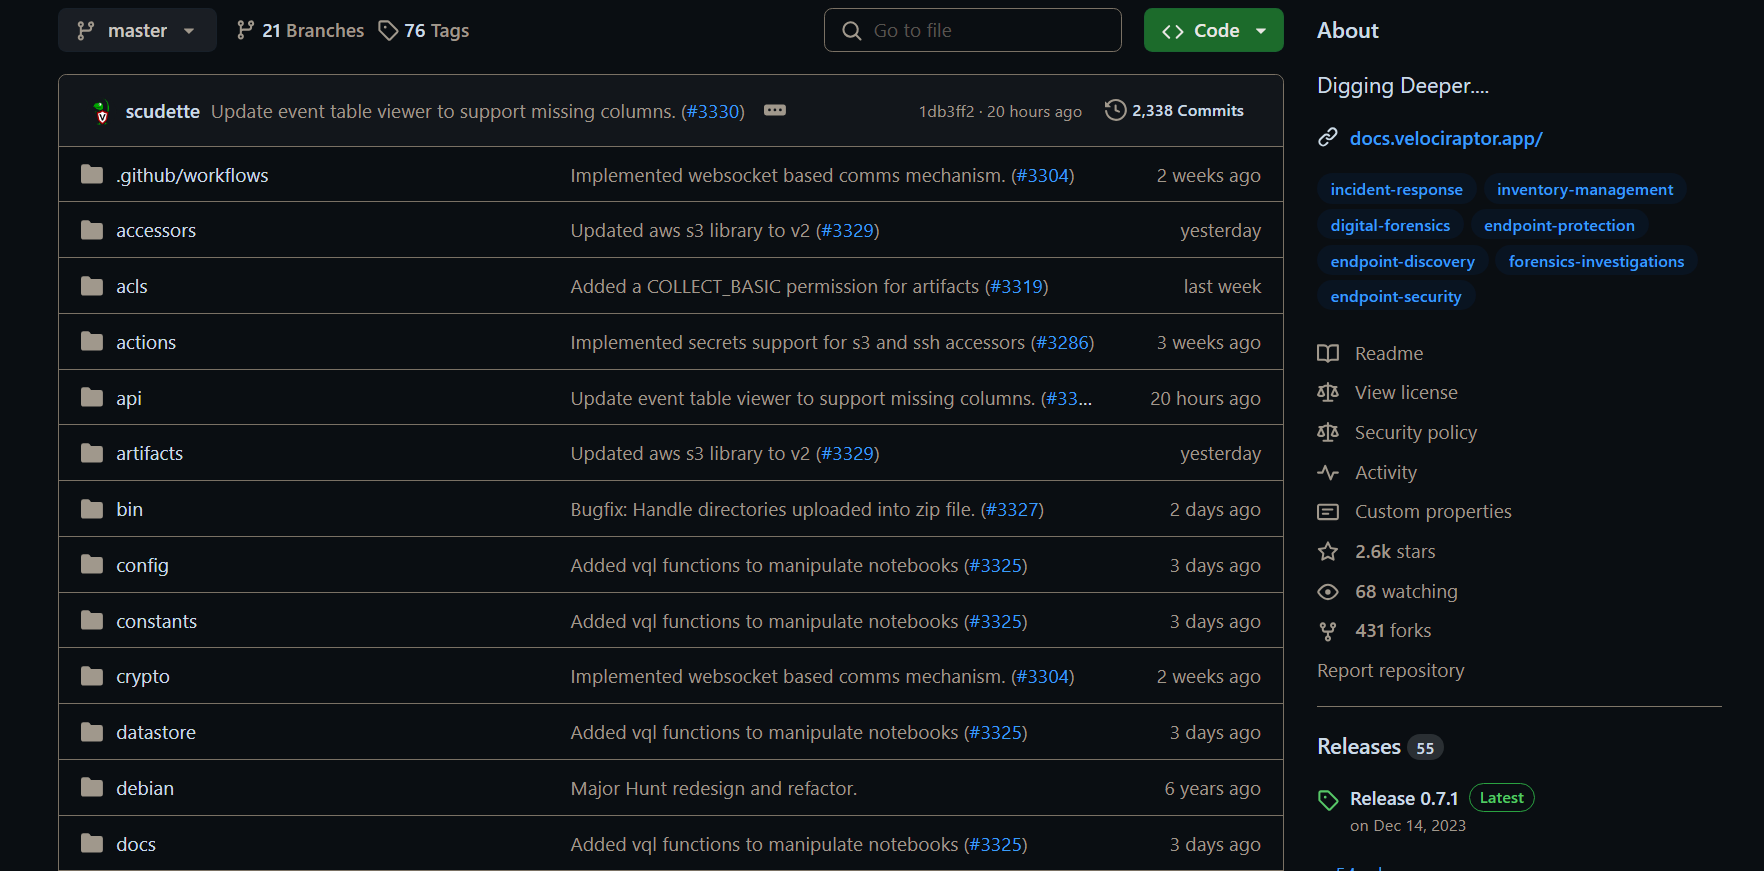
\includegraphics[width=\linewidth, center]{img/src/1.png}
    \label{fig:src1}
\end{subfigure}
\begin{subfigure}{0.48\textwidth}
    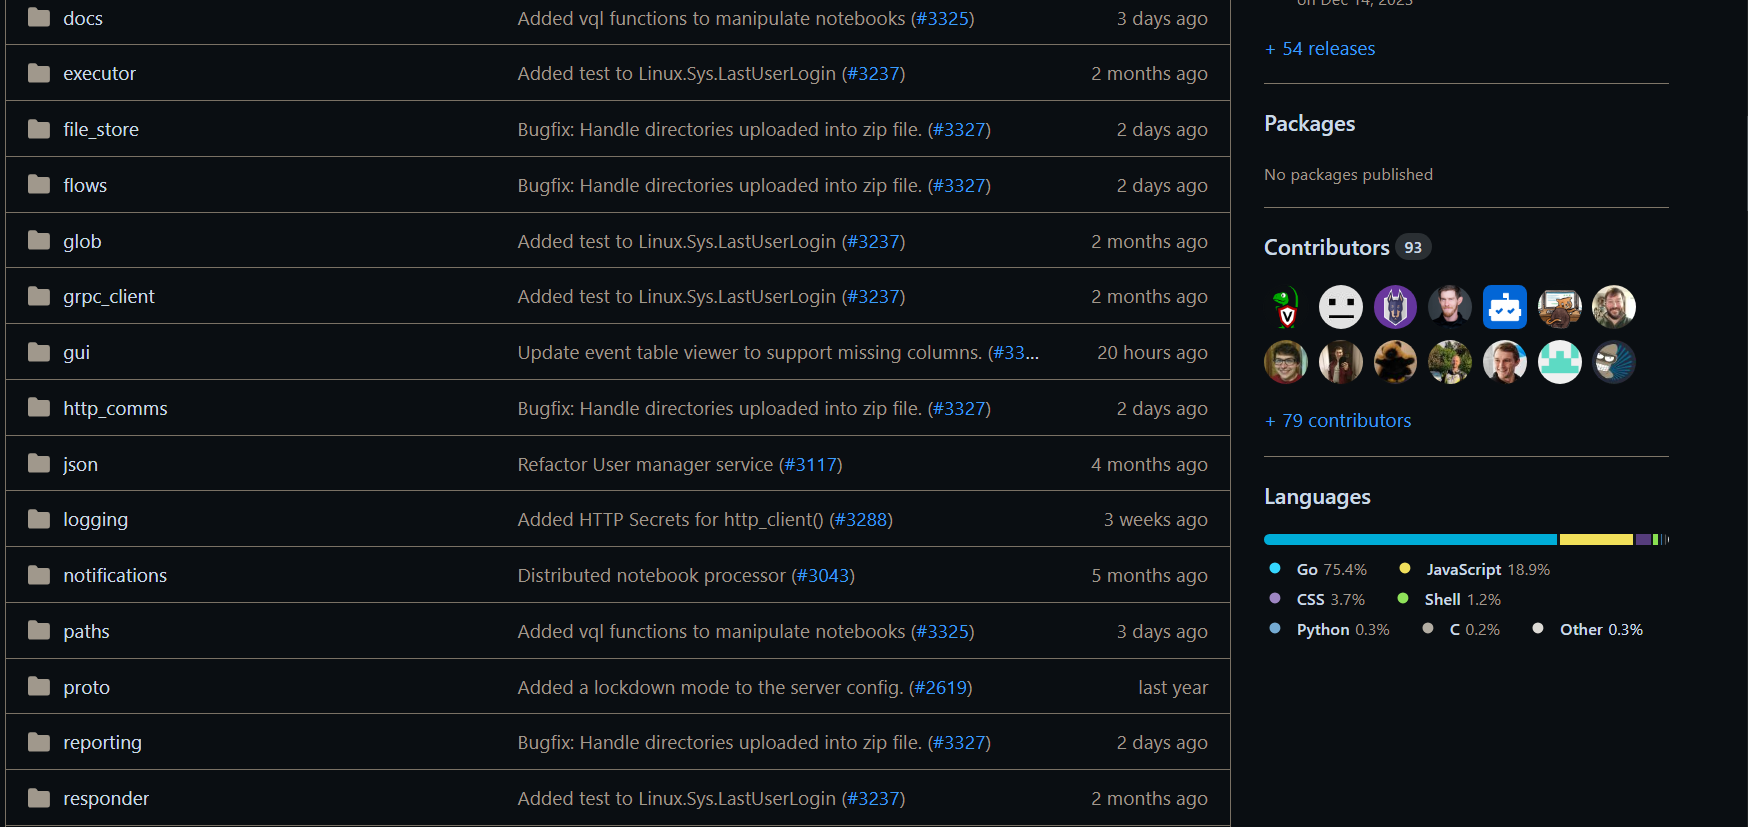
\includegraphics[width=\linewidth, center]{img/src/2.png}
    \label{fig:src2}
\end{subfigure}
\caption{Velociraptor Source Code}
\label{fig:src_code}
\end{figure}
\begin{figure}[ht]
    \centering
    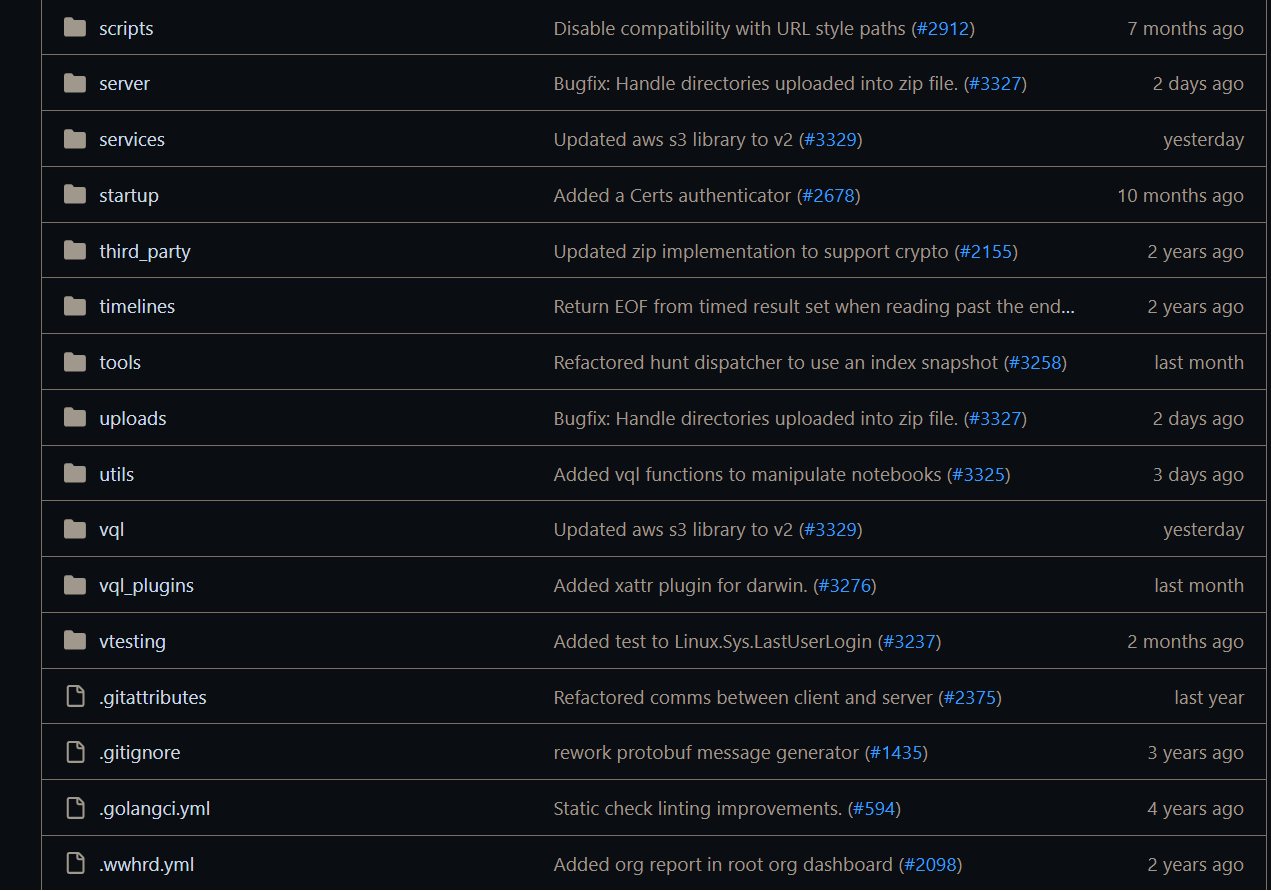
\includegraphics[width=\linewidth, scale=0.35, center]{img/src/3.png}
    \label{fig:src3}
    \caption{Velociraptor Source Code}
\end{figure}

\subsection{DFIR and Related Utility Packages}
\verb|/accessor, /acl, /actions, /artifacts,| \verb|/glob, / logging, /reporting,| \verb|/responder, /services, /timelines, /uploads| are mainly the packages that are used to perform DFIR operations such as searching, accessing, collecting and uploading files, log events, create event timelines, run different forensic services etc.

\subsection{Server, Client Administration Packages}
\verb|/api, /crypto, /grpc, /http_comms| are packages used in both the server and client side Velociraptor functionalities. \verb|/config| package is used to parse the configuration YAML files. \verb|/debian, /GUI, /server| packages provide necessary libraries for the server. 

\subsection{VQL Packages}
Packages directly related to the Velociraptor Query Language(VQL) are \\
\verb|/vql, /json, /result_sets and /vql_plugins|. These packages provide the core functionalities necessary for parsing, compiling, executing, presenting VQL queries and using different VQL plugins.

\subsection{Core Systems and Utility Packages}
\verb|/bin, /datastore, /executable,| \verb|/filestore, /flows| do the legwork of running low level services, do housekeeping etc. \verb|/constants, /path, /scripts,| \verb|/utils, /third_party| include more utility functions and libraries necessary for Velociraptor to work.

\section{Installation and Deployment}
Velociraptor can be installed in a system as a stand-alone executable or can be deployed over a centrally controlled network. Following are brief discussions on different types of Velociraptor deployments:

\subsection{Instant Velociraptor} \label{instantvel}
The Velociraptor Github repository contains latest releases with executables for Linux, Windows, Darwin. The executable can be run with \verb|gui| command line option and a local client and server will be created, with the server GUI opening in the browser. This lets the users to try out various features in their own local machine.

\subsection{Networked Deployment} As an endpoint monitoring tool, Velociraptor is usually deployed in an on-premise server, with the endpoints running Velociraptor client service. We explored and deployed Velociraptor in this method:

\begin{itemize}
    \item Interactively creating a server and client config file. The server address in client configuration should be the ip address of the server/VM that will host Velociraptor Server. 
    \begin{lstlisting}[basicstyle=\ttfamily, breaklines=true, language=bash]
        Velociraptor config generate -i
    \end{lstlisting}
    \item Creating server executable for generated \verb|server.config.yml| file:
    \begin{lstlisting}[basicstyle=\ttfamily, breaklines=true, language=bash]
        Velociraptor.exe --config server.config.yaml debian server --binary Velociraptor-v0.6.0-linux-amd64
    \end{lstlisting}
    \item Upload this server executable to a server/VM connected to the network and start the service:
    \begin{lstlisting}[basicstyle=\ttfamily, breaklines=true, language=bash]
        scp Velociraptor_server*.deb <username>@<ip address>:/tmp/
        sudo dpkg -i Velociraptor_*_server.deb
    \end{lstlisting}
    \item Visit the GUI at localhost. Since this is a self-certified SSL deployment, all connection to both GUI front-end and the endpoints are secured.
    \begin{lstlisting}[basicstyle=\ttfamily, breaklines=true, language=bash]
        https://127.0.0.1:8889/
    \end{lstlisting}
    \item Creating client installer for windows, downloading and installing it:
    \begin{figure}[ht]
    \centering
    \begin{subfigure}{0.45\linewidth}
        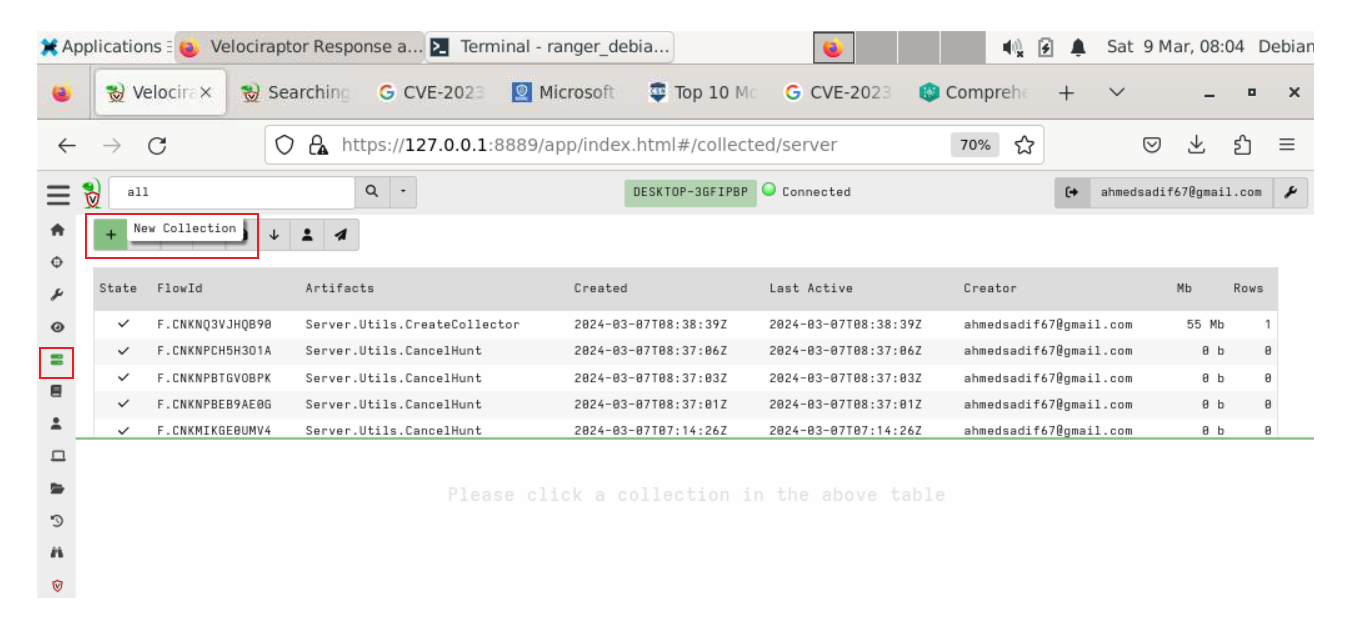
\includegraphics[width=\linewidth, center]{img/install/1.png}
        \label{fig:install1}
    \end{subfigure}
    \begin{subfigure}{0.45\linewidth}
        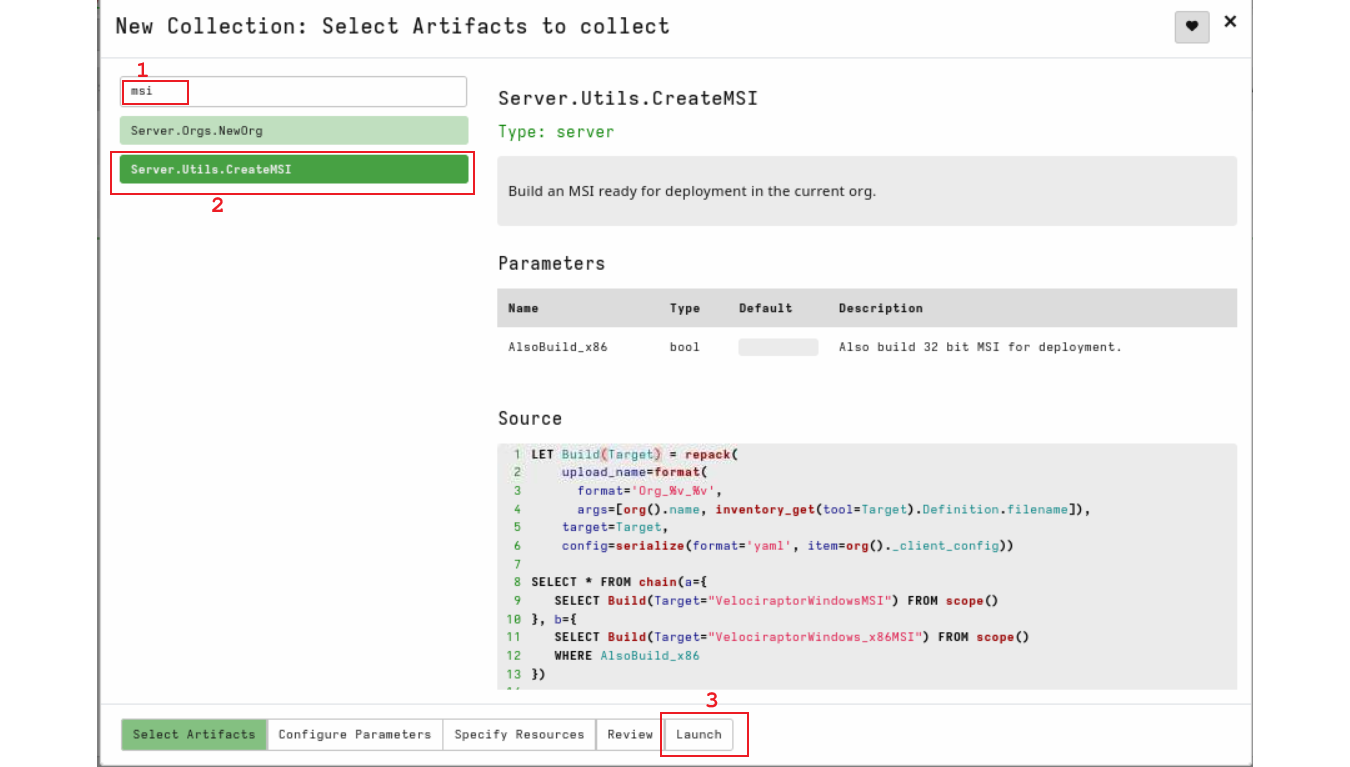
\includegraphics[width=\linewidth, center]{img/install/2.png}
        \label{fig:install2}
    \end{subfigure}

    \caption{Generating Velociraptor Client MSI From Server GUI}
    \label{fig:install}
    \end{figure}
    \begin{figure}[ht]
    \centering
    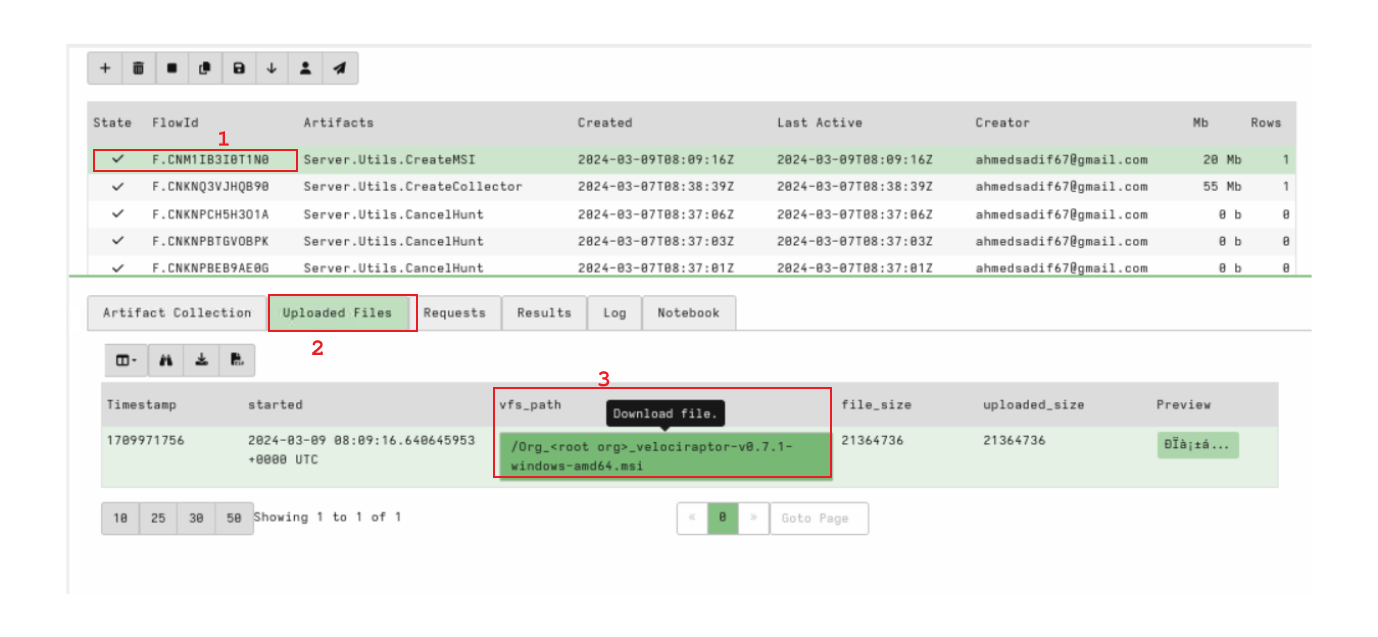
\includegraphics[width=\linewidth, center]{img/install/3.png}
    \caption{Downloading Generated MSI}
    \label{fig:install3}
    \end{figure}
    \\Or using \verb|Velociraptor.exe| as a client to test installation:
    \begin{lstlisting}[basicstyle=\ttfamily, breaklines=true, language=bash]
        Velociraptor --config client.config.yaml client -v
    \end{lstlisting}
    
\end{itemize}

\subsection{Cloud Deployment}
This is suitable when on-premise deployment is not needed and/or internet access is not blocked. However this requires a DNS name to be used for Let's Encrypt certification. Generating a config file remains similar, the additions being provisioning Let's Encrypt for SSL certification and adding an Auth provider such as Google OAuth SSO. After that, the server executable generation, setup, client generation remains almost same. 

\section{Key Features}

\subsection{Digital Evidence Collection}
Velociraptor excels in collecting digital evidence across numerous endpoints quickly and precisely, making it a valuable tool for incident response scenarios. Here's an in-depth look at this feature.

\subsubsection{Capabilities}
\begin{itemize}
    \item \textbf{Targeted Collection: }Unlike traditional methods that image entire disks, Velociraptor focuses on specific data based on your needs. This reduces collection time, minimizes storage requirements, and protects the chain of custody.
    \item \textbf{Simultaneous Acquisition: }You can collect evidence from multiple devices simultaneously, saving valuable time in large-scale investigations.
    \item \textbf{Remote Collection: } Velociraptor allows you to collect evidence remotely without physically accessing the endpoints, ideal for geographically dispersed systems or challenging environments.
    \item \textbf{Customization: }You can tailor the collection process to your specific investigation by defining what data to collect (e.g., specific files, registry keys, memory dumps) and filtering criteria (e.g., based on file names, timestamps).
    \item \textbf{VQL (Velociraptor Query Language): }
    This powerful language enables you to craft precise queries to search for specific evidence across endpoints. For example, you could use VQL to search for all files modified within the last hour, containing a specific keyword, or created by a particular user.
\end{itemize}

\subsubsection{Benefits}
\begin{itemize}
    \item \textbf{Speed: } Rapid collection of evidence is crucial in incident response, and Velociraptor significantly accelerates the process compared to traditional methods. 
    \item \textbf{Efficiency: } Targeted collection reduces unnecessary data acquisition, saving storage space and streamlining subsequent analysis.
    \item \textbf{Scalability: }Velociraptor can handle evidence collection from a large number of endpoints simultaneously, making it ideal for enterprise environments.
    \item \textbf{Accuracy: }
    VQL allows for precise searches, ensuring you only collect relevant evidence and maintain the chain of custody.
\end{itemize}

\subsubsection{Example Usage Case}
\begin{itemize}
    \item \textbf{Incident Identified: }Your organization suspects a malware infection on its network. 
    \item \textbf{Rapid Deployment: }You deploy Velociraptor to potentially affected endpoints.
    \item \textbf{Targeted Collection: }Using VQL, you create a query to search for specific files associated with the suspected malware, such as executables with specific names or registry entries created by the malware.
    \item \textbf{Simultaneous Collection: } Velociraptor gathers the identified evidence from all targeted endpoints simultaneously.
    \item \textbf{Analysis: }The collected evidence is then analyzed to confirm the presence of malware and determine the extent of the infection.
\end{itemize}
Overall, Velociraptor's efficient and targeted digital evidence collection capabilities make it a valuable tool for incident response and digital forensics investigations.

\subsection{Endpoint Activity Monitoring}

\subsubsection{Monitored Activities}

\begin{itemize}
    \item \textbf{File System Changes: }Velociraptor tracks file creation, deletion, modification, and access attempts. This can help identify suspicious activities like unauthorized file modifications or attempts to access sensitive data.
    \item \textbf{Process Activity: } It monitors running processes, including creation, termination, and resource usage. This can help detect malicious processes or unusual resource consumption indicative of potential malware or unauthorized activities.
    \item \textbf{Network Connections: }Velociraptor can monitor network connections made by endpoints, identifying unauthorized connections, suspicious communication patterns, or data exfiltration attempts.
    \item \textbf{System Logs: }It monitors various system logs, including security logs, application logs, and Windows event logs, providing valuable insights into system events and potential security issues.
\end{itemize}
\subsubsection{Benefits}
\begin{itemize}
    \item \textbf{Early Threat Detection: } By continuously monitoring endpoint activities, Velociraptor can detect potential threats in their early stages, allowing for faster response and mitigation.
    \item \textbf{Improved Security Posture: } Continuous monitoring helps maintain a vigilant security posture by identifying potential vulnerabilities and suspicious activities before they escalate into major incidents.
    \item \textbf{Forensic Analysis: }The collected data from monitored activities can be used for forensic analysis in case of a security incident, aiding in identifying the root cause and scope of the attack.
\end{itemize}
\subsubsection{Example Usage Case}
\begin{itemize}
    \item \textbf{Suspicious Process: } Velociraptor detects a new process running on an endpoint that consumes unusually high CPU resources.
    \item \textbf{Investigation: }The security team investigates the process and finds it has no legitimate purpose and exhibits characteristics of malware.
    \item \textbf{Rapid Response: } The team takes immediate action to contain the threat, such as isolating the infected endpoint and preventing further damage.  
\end{itemize}
Overall, Velociraptor's continuous endpoint activity monitoring plays a crucial role in proactive threat detection, improving your organization's security posture and enabling rapid response to potential incidents.
\subsection{Forensic Analysis}
Velociraptor goes beyond simply collecting digital evidence. It empowers investigators to analyze the collected data for malicious activity, malware presence, and other suspicious actions, aiding in forensic investigations.
\subsubsection{Analysis Tools}
\begin{itemize}
    \item \textbf{File Analysis: }Velociraptor can analyze files for various indicators of compromise (IOCs), such as suspicious file hashes, embedded malicious code, and known malware signatures.
    \item \textbf{Memory Analysis: }It allows analysis of memory dumps to identify potentially hidden malware processes, injected code, and other volatile artifacts that might not be evident on disk.
    \item \textbf{Registry Analysis: } Velociraptor enables investigators to examine the Windows Registry for suspicious entries created by malware or unauthorized modifications.
    \item \textbf{Network Analysis: }Network traffic captured by Velociraptor can be analyzed to identify unusual communication patterns, data exfiltration attempts, or connections to known malicious domains.
    \item \textbf{Log Analysis: }System logs collected during monitoring can be analyzed for suspicious events, failed login attempts, or error messages indicative of security incidents.
\end{itemize}
\subsubsection{Benefits}
\begin{itemize}
    \item \textbf{Efficiency: } VQL and integration with other tools streamline the analysis process, saving investigators valuable time.
    \item \textbf{Accuracy: }Precise searches and analysis capabilities ensure investigators focus on relevant evidence, leading to more accurate conclusions.
    \item \textbf{Comprehensiveness: }Velociraptor offers diverse analysis tools, enabling a comprehensive investigation across various digital artifacts.
    \item \textbf{Collaboration: }The centralized storage and visualization features facilitate collaboration among investigators, allowing for efficient case management.
\end{itemize}
\subsubsection{Example Usage Case}
\begin{itemize}
    \item \textbf{Incident Response: }Following a suspected ransomware attack, investigators use Velociraptor to collect evidence from affected endpoints.
    \item \textbf{File Analysis: } Analysis of collected files reveals files encrypted with a known ransomware signature, confirming the attack.
    \item \textbf{Memory Analysis: } Memory analysis uncovers a hidden process responsible for encrypting files, further aiding in identifying the specific malware variant.
    \item \textbf{Network Analysis: }Network traffic analysis reveals connections to a known command-and-control server used by the ransomware, providing crucial intelligence for tracking the attackers.
\end{itemize}
By offering a robust set of analysis tools and functionalities, Velociraptor empowers investigators to efficiently and effectively analyze evidence, leading to faster incident resolution and improved forensic investigations.
\subsection{Threat Hunting Capabilities}
Velociraptor empowers security professionals with advanced threat hunting capabilities to proactively identify and respond to potential threats before they cause significant damage.
\subsubsection{Pre-built Queries}
Velociraptor comes with a comprehensive library of pre-built queries targeting known threats, vulnerabilities, and suspicious activities. These queries leverage community-developed expertise and threat intelligence, allowing you to quickly hunt for specific threats without starting from scratch.
Example:
\begin{itemize}
    \item Identifying unauthorized remote desktop connections.
    \item Searching for specific malware signatures in memory.
    \item Detecting suspicious PowerShell activity.
\end{itemize}
\subsubsection{Custom Query Creation}
Velociraptor empowers you to create custom queries using VQL (Velociraptor Query Language). VQL is a powerful language tailored for searching and analyzing endpoint data.
Example:
\begin{itemize}
    \item Combine various data sources like file system, registry, memory, and network connections for comprehensive threat hunting.
    \item Filter and search for specific indicators of compromise (IOCs) based on your organization's specific needs and threat landscape.
    \item Develop custom queries to hunt for emerging threats and unknown malware not covered by pre-built queries.
\end{itemize}
\subsubsection{Benefits}
\begin{itemize}
    \item \textbf{Proactive Security: }By proactively hunting for threats instead of waiting for them to manifest, you can identify potential security issues before they escalate into major incidents.
    \item \textbf{Improved Detection Rates: } Utilizing both pre-built and custom queries allows you to cast a wider net and detect a broader range of potential threats compared to traditional security solutions.
    \item \textbf{Faster Response: }Early detection through threat hunting enables you to take timely action and mitigate potential threats before they cause significant damage or data loss.
    \item \textbf{Customization: }The ability to create custom queries caters to your organization's specific needs and threat landscape, allowing for targeted hunting efforts.
\end{itemize}
\subsubsection{Example Usage Case}
\begin{itemize}
    \item Security analysts learn about a new phishing campaign targeting their organization through threat intelligence reports.
    \item They create a custom VQL query to search for specific indicators associated with the campaign, such as suspicious email attachments or registry modifications by the malicious payload. 
    \item Velociraptor executes the query across all endpoints, identifying potentially compromised systems.
    \item Security teams can then take immediate action to isolate the affected systems, remediate the threat, and prevent further harm.
\end{itemize}
Overall, Velociraptor's threat hunting capabilities offer a powerful solution for proactive security, empowering you to identify and address potential threats before they cause significant damage.
\subsection{Centralized Storage}
Velociraptor offers a centralized storage solution for all the digital evidence and data collected during investigations and endpoint monitoring.
\subsubsection{Unlimited Retention}
Unlike traditional methods that might have storage limitations, Velociraptor stores collected data indefinitely. This enables investigators to revisit and analyze evidence even after an incident has been resolved, which can be crucial for:
\begin{itemize}
    \item \textbf{Identifying connections to past incidents: }By analyzing historical data, investigators might discover connections between seemingly unrelated events, leading to a broader understanding of an attacker's campaign or uncovering previously undetected threats.
    \item \textbf{Compliance with regulations: } Certain regulations might mandate retaining forensic data for extended periods. Centralized storage with unlimited retention ensures compliance with such regulations.
    \end{itemize}
\subsubsection{Improved Accessibility}The centralized storage makes collected data readily accessible to authorized investigators from any location with an internet connection. This eliminates the need to physically access individual devices or maintain copies of collected data in different locations, streamlining collaboration and investigation workflows.
\subsubsection{Efficient Management}Centralized storage simplifies data management tasks such as: 
\begin{itemize}
    \item \textbf{Backups: }Implementing a centralized backup strategy ensures data protection in case of hardware failures or other unforeseen events.
    \item \textbf{Archiving: } Older data can be archived to free up space in the primary storage while still being accessible for historical analysis.
    \item \textbf{Access control: }Granular access controls can be implemented to ensure only authorized personnel can access sensitive data, maintaining data security and integrity.
\end{itemize}
\subsubsection{Enhanced Collaboration} Having all evidence stored centrally fosters collaboration among investigators. They can easily share and analyze data, discuss findings, and work together to reach conclusions efficiently.
\subsection{Example Usage Case}
\begin{itemize}
    \item An organization experiences a data breach in 2023.
    \item Investigators use Velociraptor to collect and store evidence from the affected systems.
    \item In 2024, the organization identifies suspicious activity that might be related to the 2023 breach.
    \item Investigators can easily access the stored evidence from 2023 using Velociraptor's centralized storage and analyze it in the context of the new findings, potentially uncovering crucial connections and leading to a more comprehensive understanding of the incident.
\end{itemize}
Overall, Velociraptor's centralized storage with unlimited retention offers a valuable asset for digital forensics and incident response investigations, enabling efficient data management, improved accessibility, and facilitating comprehensive analysis even after an incident is seemingly resolved.
\section{Some Features In Detail}

\subsection{Basic Usage and Introduction}

\subsubsection{A Tour of the GUI}
The Velociraptor GUI is the front-end for the server side of a Velociraptor deployment. It is made with React and thus highly responsive. Some commonly used tabs and pages of the GUI are discussed below, with relevant image parts boxed with red boundary:
\begin{itemize}
    \item \textbf{Homepage:} The homepage lists the server status, along with some other basic information. The sidebar is available to be expanded at any page, and acts as the navigation anchor of the GUI.
    \begin{figure}[H]
        \centering
        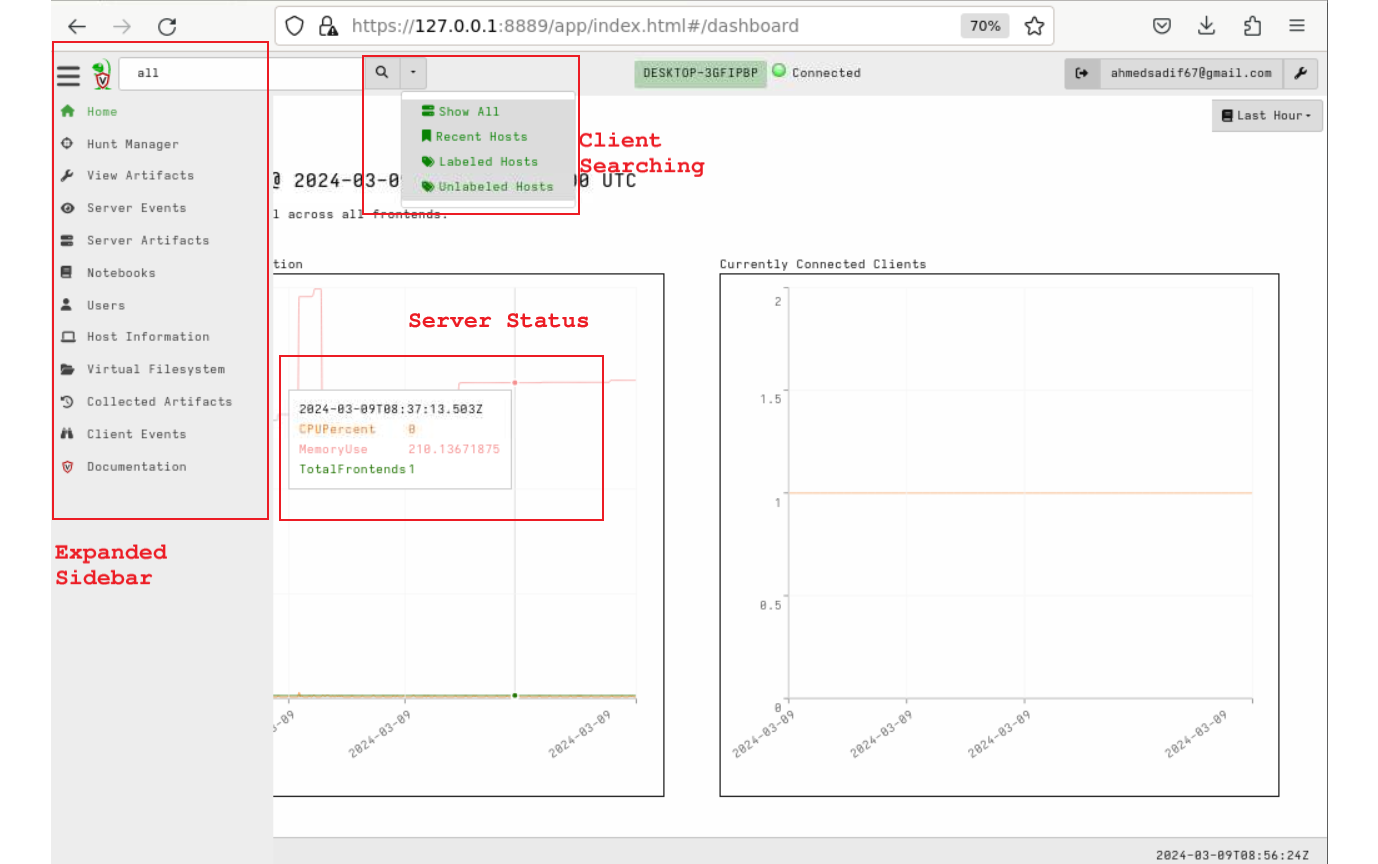
\includegraphics[scale=0.31]{img/GUI/home/1.png}
        \caption{Home Page}
        \label{fig:GUIhome1}
    \end{figure}
    \item  \textbf{Artifacts:} Artifacts are multiple VQL queries wrapped in a YAML file, with provision for adding parameters, description etc.
    \begin{figure}[H]
        \centering
        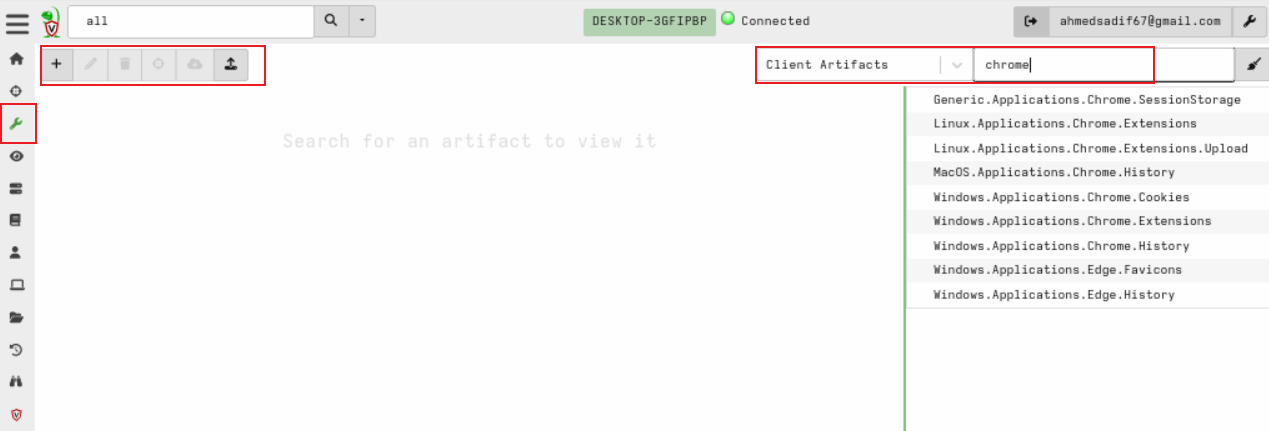
\includegraphics[scale=0.35]{img/GUI/home/6.png}
        \caption{Artifacts Viewing Tab}
        \label{fig:GUIhome6}
    \end{figure}
    \begin{figure}[H]
        \centering
        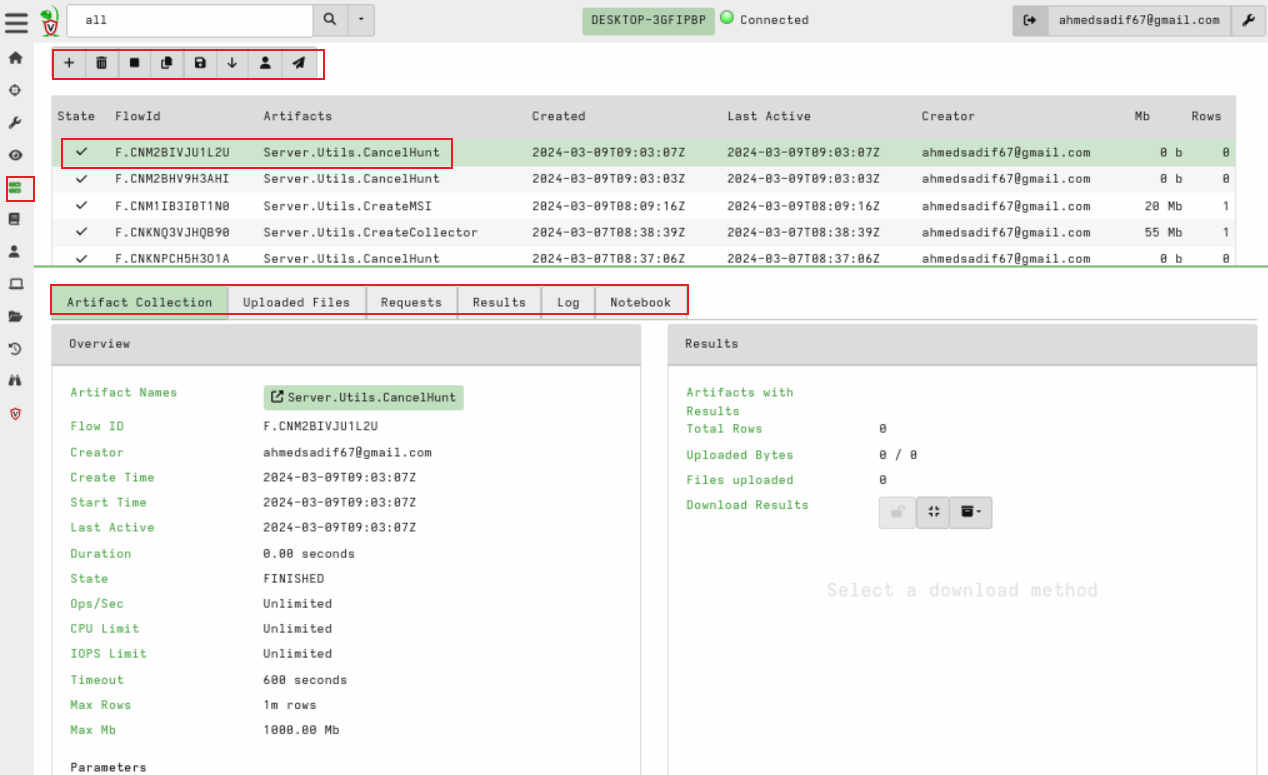
\includegraphics[scale=0.35]{img/GUI/home/7.png}
        \caption{Server Side Artifacts Tab}
        \label{fig:GUIhome7}
    \end{figure}
    \item \textbf{Notebook:} Notebook provides a way to run VQL queries along with adding information in markup language.
    \begin{figure}[H]
        \centering
        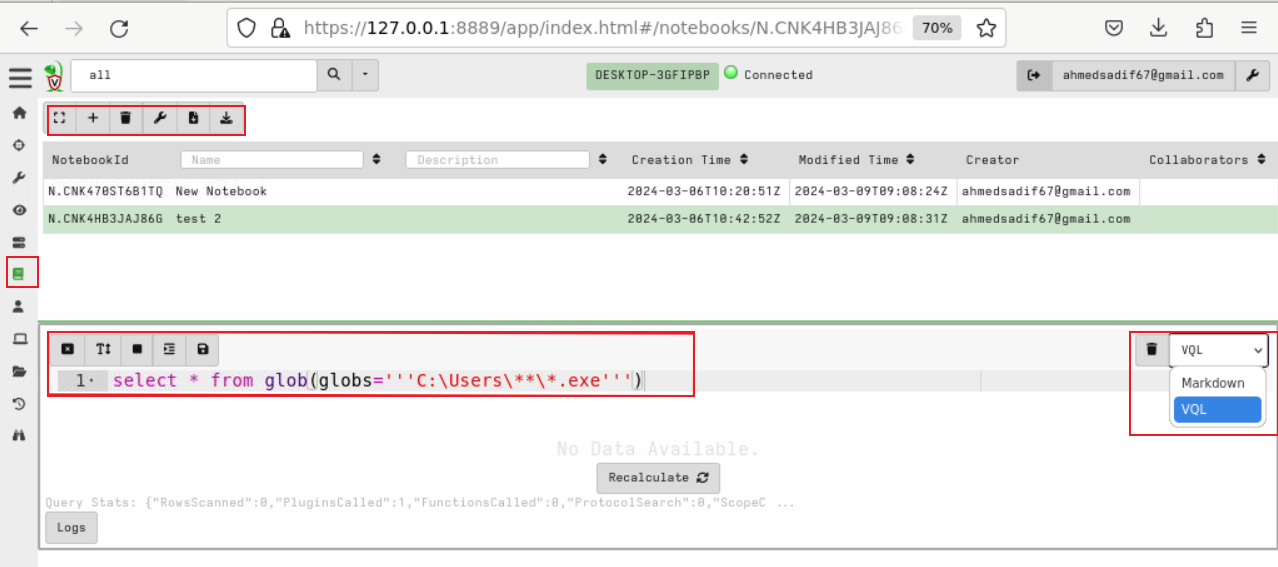
\includegraphics[scale=0.35]{img/GUI/home/8.png}
        \caption{Notebooks Tab}
        \label{fig:GUIhome8}
    \end{figure}
    \item \textbf{Hunt Tab:} Hunts are how endpoints receive command from server to collect, streamline and possibly analyze forensic data and report back to server.
    \begin{figure}[H]
        \centering
        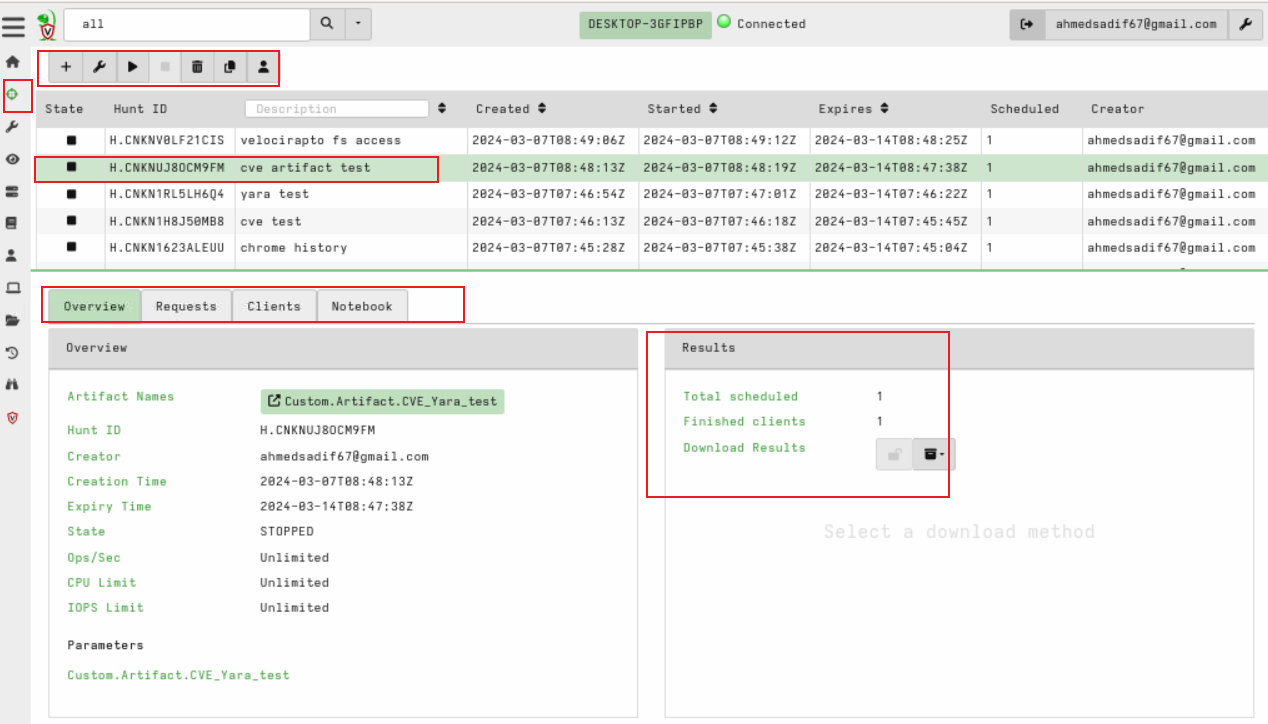
\includegraphics[scale=0.35]{img/GUI/home/5.png}
        \caption{Hunts Tab}
        \label{fig:GUIhome5}
    \end{figure}
    \item \textbf{Client Information Tab:} Selecting a single client enables this and following tabs, allowing user to view from server important client information.
    \begin{figure}[H]
        \centering
        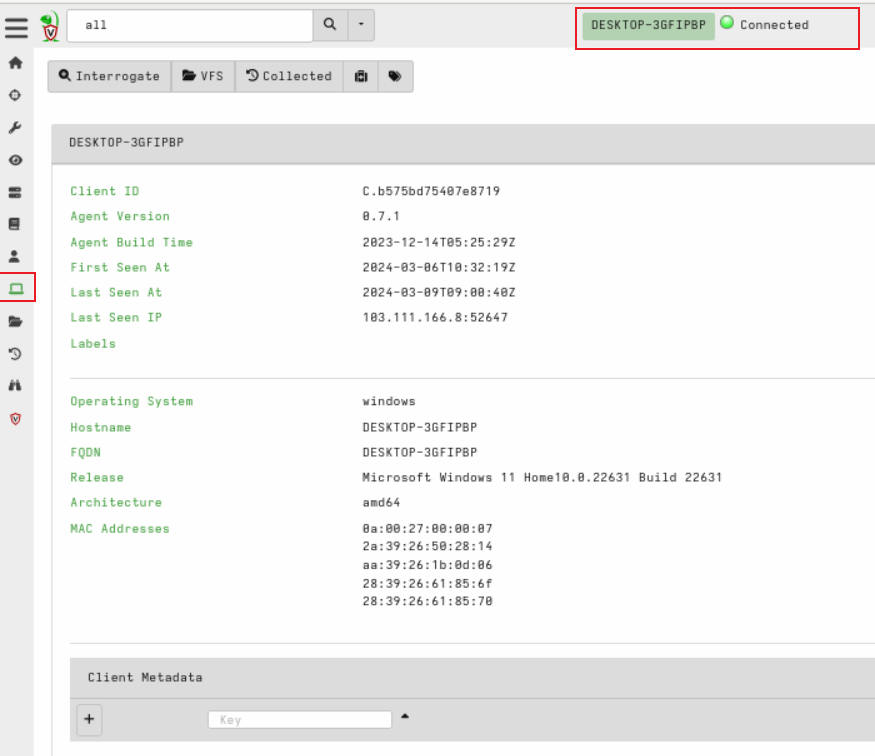
\includegraphics[scale=0.35]{img/GUI/home/3.png}
        \caption{Client Information Tab}
        \label{fig:GUIhome3}
    \end{figure}
    \item \textbf{Virtual File System Tab:} This tab allows user to explore the file system of a selected endpoint.
    \begin{figure}[H]
        \centering
        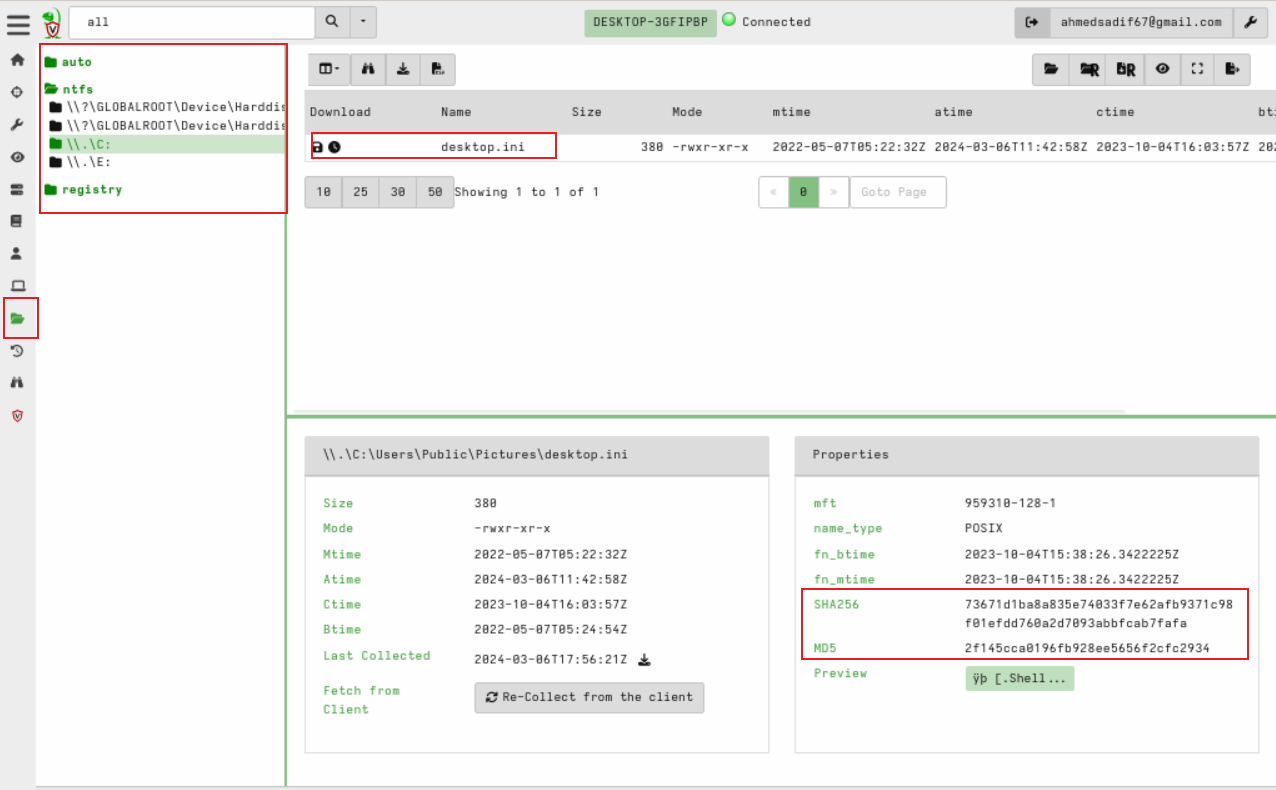
\includegraphics[scale=0.35]{img/GUI/home/4.png}
        \caption{File System Tab}
        \label{fig:GUIhome4}
    \end{figure}

\end{itemize}

\subsubsection{Velociraptor Query Language}\label{vql}
The Velociraptor Query Language(VQL) allows users to pose structured, succinct queries to the endpoints or the server and then streamline the results. The language is similar to the well known Structured Query Language(SQL), in fact the most common syntax is:
\begin{lstlisting}[basicstyle=\ttfamily, breaklines=true, language=SQL]
        SELECT ... FROM ... WHERE
\end{lstlisting}
However, it is much simpler, with no \verb|JOIN| or \verb|HAVING| clause. The resultant rows are not from any pre-generated tables, rather VQL plugin outputs. VQL uses lazy evaluation, such that only after necessary filtering of output rows from plugins that a query is parsed. The power of VQL lies in the numerous available plugins that can be leveraged to inspect, extract and manipulate client state from server.
\\
A powerful feature of VQL is the \verb|foreach| plugin:
\begin{lstlisting}[basicstyle=\ttfamily, breaklines=true, language=SQL]
        SELECT ... FROM foreach( 
            rows = { SELECT ... FROM ... WHERE},
            query = { SELECT ... FROM ... WHERE},
            workers = integer
                )
\end{lstlisting}
For each row that is fetched from the \verb|rows| query, the \verb|query| is run and result is further filtered in the \verb|SELECT ... FROM foreach| query. It is possible make \verb|foreach| execution parallel, by specifying number of workers.
\\
VQL by itself is just using the Velociraptor engine to run various plugins. Thus VQL can be extremely powerful and can be extended easily. For example \verb|Admin.Client.Upgrade.Windows| artifact(\ref{artifacts}) can be used to push upgrades to endpoint OS from server!
\\
\textbf{Notebooks:}\label{notebooks} Notebooks are the way to write VQL queries in the GUI, that can be commented on with markdown. Notebooks are the easiest way to analyze collected data in server, so each hunt and flow has its own notebook. It is also possible to create own notebook for fleshing out any new idea in VQL.
\begin{figure}[ht]
    \centering
    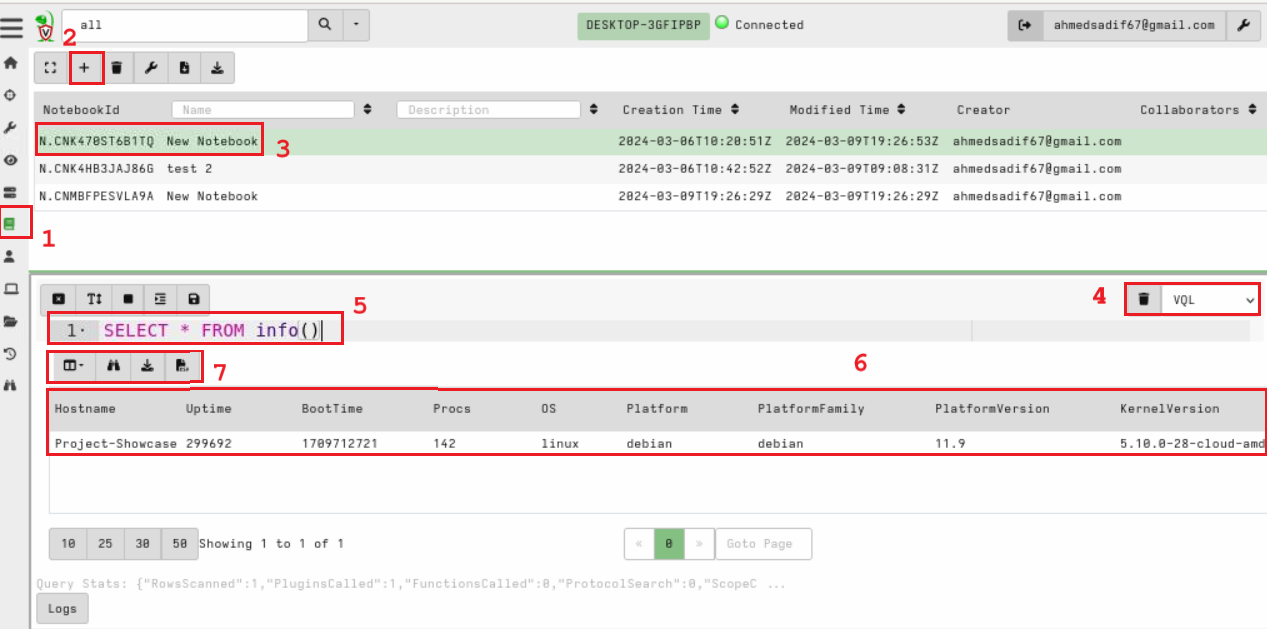
\includegraphics[width=\linewidth, scale=0.5, center]{img/vql/1.png}
    \caption{A Notebook}
    \label{fig:notebook1}
\end{figure}

\subsubsection{Using Artifacts}\label{artifacts}
Artifacts are abstractions over some related VQL queries, that provide a user to collect some useful forensic data without necessarily knowing VQL. Artifacts are written in YAML, and accessible from both view artifacts tab(figure \ref{fig:GUIhome6}) and server artifacts tab(figure \ref{fig:GUIhome7}). Each artifact contains human readable description and needed parameters to run the queries. Artifacts are readily customizable and new artifacts can be easily written.
\\ 
Artifacts provide the core of Velociraptor functionalities, in that everything both visible in the GUI and executable through hunts are artifacts. Velociraptor is essentially the engine that runs the VQL queries in artifacts, see \ref{fig:GUIhome7}. As such, artifacts are first compiled into VQL, then pushed to endpoints so that result can be calculated and relayed back to server.
\begin{figure}[ht]
    \centering
    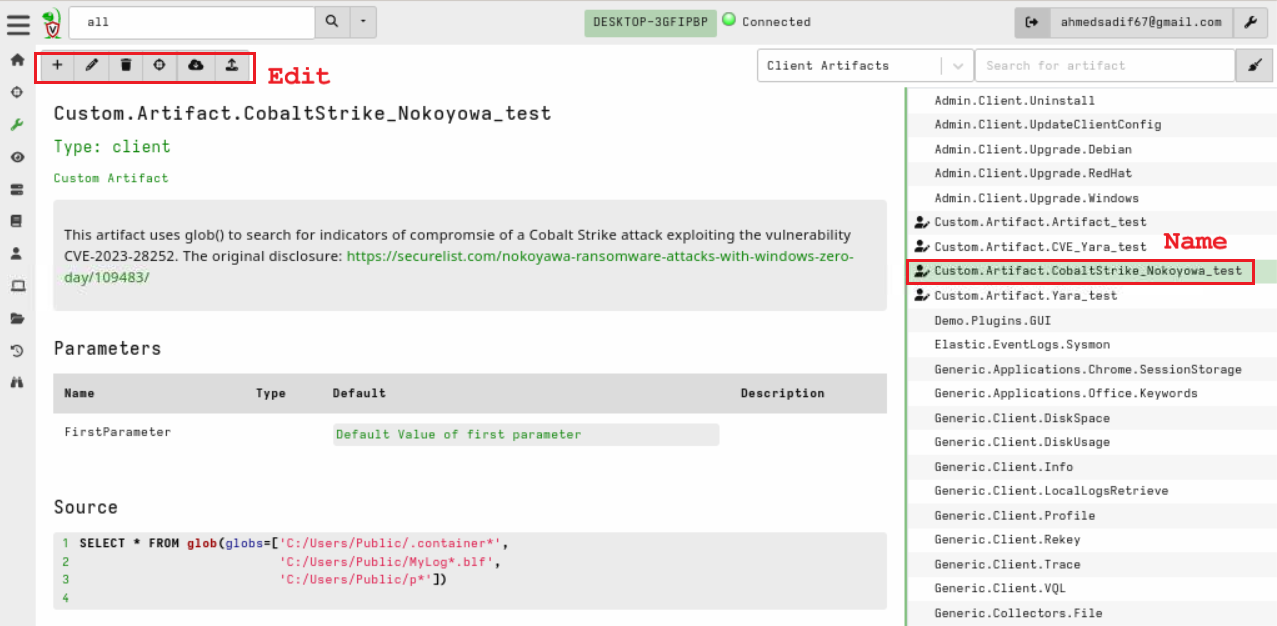
\includegraphics[width=\linewidth, scale=0.5, center]{img/vql/2.png}
    \caption{A Custom Artifact}
    \label{fig:artifact1}
\end{figure}

\subsubsection{Hunts}
Velociraptor is easily scalable, with servers monitoring 5-10k endpoints easily. The preferred way of dealing with endpoints is through hunts. Hunts are scheduled tasks that are passed to selected endpoints immediately after being setup. Endpoints perform specified tasks in the hunt -- usually multiple artifacts -- and relay back any results to server, see \ref{fig:GUIhome5}. Hunts are given expiry dates, as such any eligible endpoint will receive the hunt during this time and execute it. Post processing of hunt collection can be done in the hunt notebook.
\\
Since VQL queries make it possible to do much of the analysis in endpoints, amount of collected data is usually of manageable amount. However, due to the fast nature of VQL execution, in a deployment with large numbers of client, a single hunt may quickly acquire very large amount of data so caution is required. It is recommended to run collection artifacts in clients only after determining which endpoints are needed to be examined and what needs to be actually collected in any hunt. 

\subsection{Forensics}
Using the basic knowledge of VQL queries, artifacts and hunts, users can perform powerful digital forensic operations in endpoints in large scale without needing much central processing of data. In this and the following section some common DFIR techniques are shown using Velociraptor.
\\
Most example codes are run on the notebook(\ref{notebooks}) tab in the GUI(figure \ref{fig:GUIhome8}). A deployment of the instant Velociraptor type (\ref{instantvel}) can be used to try them out.


\subsubsection{Filename Searching}\label{glob}
The \verb|glob()| VQL plugin is the foremost tool to search filenames in endpoints. This lets the user to run wildcard search, with recursive path resolution. \verb|glob()| automatically creates optimizations for multiple path search.
\begin{lstlisting}[basicstyle=\ttfamily, breaklines=true, language=SQL]
        SELECT * FROM glob(
                    globs=['<path>', ...]|url(scheme, path, fragment),
                    [accessor="accessor name"]
                    )
\end{lstlisting}
\begin{figure}[ht]
    \centering
    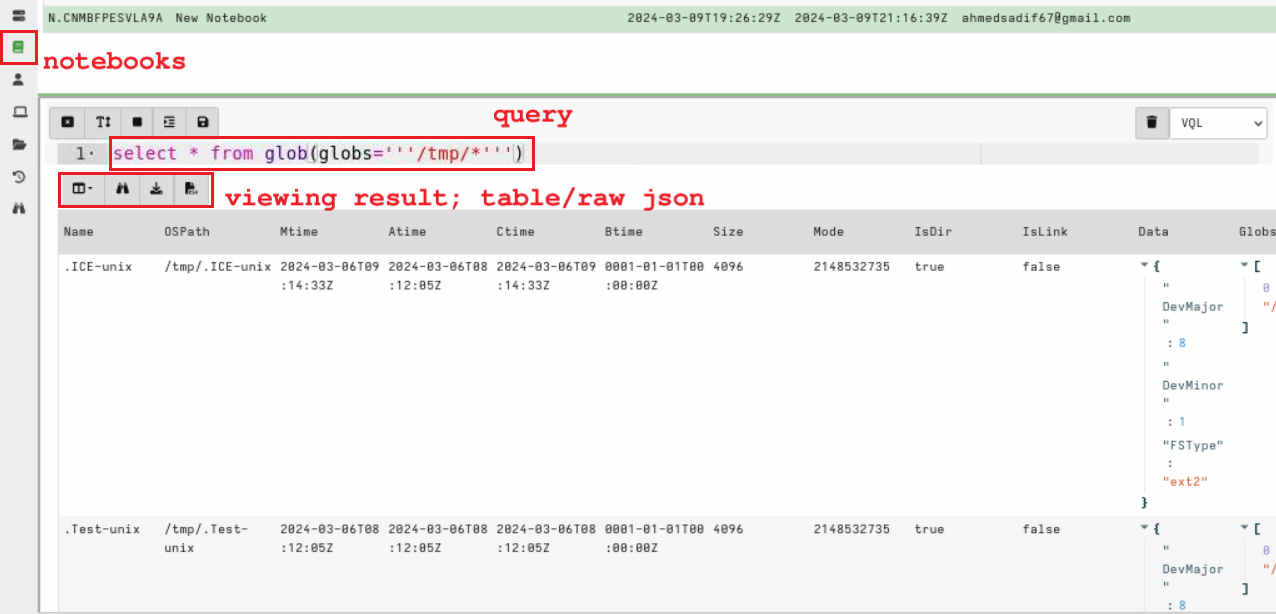
\includegraphics[width=\linewidth, scale=0.35, center]{img/forensic/glob1.png}
    \caption{A glob() Query}
    \label{fig:glob1}
\end{figure}
Since registries are hierarchical like files in Windows, it is possible to search in the registry values using \verb|glob()|. Velociraptor provides accessors for the endpoints file system and registry.

\subsubsection{File System} 
Accessing the file system at each endpoint is possible through the virtual file system tab(figure \ref{fig:GUIhome4}). Velociraptor can use the endpoints file system as presented, with the \verb|auto| accessor. However, for more extensive DFIR purposes, the \verb|ntfs| accessor is more suitable. The relevant accessors, plugins and artifacts are listed  below:
\begin{itemize}
    \item \textbf{ntfs Accessor:} This directly parses the \verb|$MFT| table at endpoint and traverses all files in system, even those hidden by api. This accessor can be used instead of \verb|file| to have deeper access to endpoint files ystem in any VQL plugin that accepts an accessor such as \verb|glob()| (\ref{glob}).
    \item \textbf{parse\_mft() Plugin:} This plugin can read the \verb|$MFT| of a NTFS disk and retrieve data from each entry.
    \begin{lstlisting}[basicstyle=\ttfamily, breaklines=true, language=SQL]
        SELECT * FROM parse_mft(
                            filename="<filename>",
                            accessor="ntfs"
                            )
        WHERE ...
    \end{lstlisting}
    \item \textbf{parse\_ntfs() Plugin:} This accepts an MFT id and outputs details about each MFT entry.
    \item \textbf{parse\_ntfs\_i30() Plugin:} This is a powerful tool to examine the real timestamps of files and their attributes. This and \verb|USN Journal| can be used to detect timestomping or malicious actors modifying file timestamps.
    \begin{lstlisting}[basicstyle=\ttfamily, breaklines=true, language=SQL]
        SELECT * FROM foreach(
            row={
            SELECT ... as MFT
            FROM glob(globs=DirectoryGlobs, accessor="ntfs") WHERE ...
            },
            query={
            SELECT ...
            FROM parse_ntfs_i30(device=FullPath, inode=MFT)
            }
        )
    \end{lstlisting}
    \item \textbf{parse\_usn() Plugin:} \verb|USN Journals| are the metadata about file system changes that are kept for journalling and backup. These are highly used source for getting timestamp of events and creating timelines. \verb|parse_usn()| takes the name of a device and returns each USN entry. Windows.Forensics.Usn artifact can be used to collect the whole \verb|USN Journal| for further use.
    \begin{lstlisting}[basicstyle=\ttfamily, breaklines=true, language=SQL]
        SELECT ... FROM parse_usn(device="<name>") WHERE ...
    \end{lstlisting}
    \item \textbf{upload() Plugin:}\label{upload} Using the \verb|upload()| plugin, a selected file can be uploaded using its file path, an accessor and optionally a new name.
\end{itemize}

\subsubsection{Content Searching}
The contents of any file are what ultimately investigated in any DFIR process. Velociraptor has support for YARA and Sigma searching. Yara is well known for its simultaneous searches through binary data for patterns specified in the following format:

\begin{lstlisting}[basicstyle=\ttfamily, breaklines=true]
        rule X {
            strings: 
                $<name> = "<string>" [options] | /<regex>/i
            condition:
                <boolean condition>
            }
\end{lstlisting}
VQL has the plugins \verb|yara()| to search bulk binary data in disk and \verb|proc_yara()| to search the process memories.
\begin{lstlisting}[basicstyle=\ttfamily, breaklines=true, language=SQL]
        LET YaraRule = '''<yara rule>'''

        SELECT * FROM foreach(
                row={
                    SELECT ... FROM ... WHERE ...
                }, 
                query={
                    SELECT str(str=String.Data) AS Hit,
                            String.Offset AS Offset,
                            FileName
                    FROM yara(files=FullPath, rules=YaraRule)
                }
            )
\end{lstlisting}
A thing to keep in mind is that, yara hits should always be considered with caution and more contextual data should be collected.

\subsubsection{Execution Histories}
All operating systems keep track of all running processes, their execution timestamps, accessed files etc. In Windows, there are many detailed types of such record. For DFIR purpose, these are very useful for creating timelines, causal relations etc. Velociraptor provides a rich set of preset artifacts(\ref{artifacts}) to access and analyze these data.
\begin{itemize}
    \item \textbf{Windows.Forensics.Prefetch, Windows.Timelines.Prefetch:} These work on the Prefetch Files of Windows. Prefetch files are Windows' way of tracking user startup activity. These tow artifacts can show records of all prefetch file entries with timestamps.
    \item \textbf{Windows.Forensics.Bam:} This artifact parses the binary data stored by the Background Activity Monitor service of Windows.
    \item \textbf{Windows.Registry.AppCompatCache:} Shims are compatibility layers over older API. Windows changes binaries if needed for compatibility and stores the modification metadata in the shim cache. This artifact parses this cache.
    \item \textbf{Windows.System.Amcache:} Thie artifact uses \verb|raw_reg| accessor to parse raw registry file type cache containing process creation timeline by the Windows Application Experience Service.
    \item \textbf{Windows.Forensics.SRUM:} This artifact tries to parse the System Resource Monitor database poweirng the Task Monitor in Windows. Since this database is not well documented, not all data can be extracted.
\end{itemize}

\subsubsection{Processes and Memory}
Traditional memory dumps suffer from the fact that a large dump -- often over network -- will inevitably disturb the volatile data in memory. Velociraptor tries to avoid this by using apis that read memory unobtrusively. Plugins and artifacts commonly used are:
\begin{itemize}
    \item \textbf{wmi() Plugin:} This uses the well known Windows Management Instrumentation api with WMI Query Language(WQL). Tools like \verb|wmie2| can be used to explore and decide what should be searched.
    \begin{lstlisting}[basicstyle=\ttfamily, breaklines=true, language=SQL]
        SELECT ... FROM wmi(query="SELECT ... FROM ... WHERE ...") WHERE ...
    \end{lstlisting}
    \item \textbf{Windows.Detection.Mutants Artifact:} This artifact enumerates current mutants(mutexes) in memory. Mutants are well known mechanism used by malware to avoid multi instance problem. Thus mutants can be further searched for hits and malware identified.
\end{itemize}
Processes can be investigated with various Velociraptor plugins and artifacts:
\begin{itemize}
    \item \textbf{pslist() Plugin:} This versatile plugin can be used to simply list all processes, or run complex filtering and subqueries to find process memories.
    \item \textbf{Windows.System.Pstree Artifact:} This artifact attempts to create a process tree. However, malware can easily spoof process calls and thus the results are not always useful.
    \item \textbf{vad() Plugin:} This plugin shows all memory regions and the filename they are mapped to, if any. Together with \verb|pslist()|, this can be used to find process memory mappings. 
    \begin{lstlisting}[basicstyle=\ttfamily, breaklines=true, language=SQL]
        LET processes = SELECT ..., Pid FROM pslist()
                        WHERE ...
        SELECT * FROM foreach(
                        row=processes,
                        query={
                                SELECT ...
                                FROM vad(pid=Pid)
                                GROUP BY ...
                            }
                    ) WHERE ...
    \end{lstlisting}
\end{itemize}

\subsubsection{Event Logging}
Windows events are stored in binary \verb|.evtx| format, with advantages for the system, but disadvantages to the DFIR investigator. Collecting all \verb|.evtx| files will not collect the event messages. So some improvisation is required. Plugins and artifacts working with events include:
\begin{itemize}
    \item \textbf{parse\_evtx() Plugin:} This parses any \verb|.evtx| file.
    \item \textbf{Windows.EventLogs.Modifications Artifact:} This looks for any modification of the logging controller registry keys and thus finding out about potential malicious activity.
    \item \textbf{watch\_etw() Plugin:} Event Tracing for Windows(ETW) is the mechanism for providing the logs from  producers to consumers. \verb|watch_etw()| thus can watch for any event in endpoint and inform server of it in real time. 
\end{itemize}
 \begin{figure}[ht]
    \centering
    \begin{subfigure}{0.45\linewidth}
        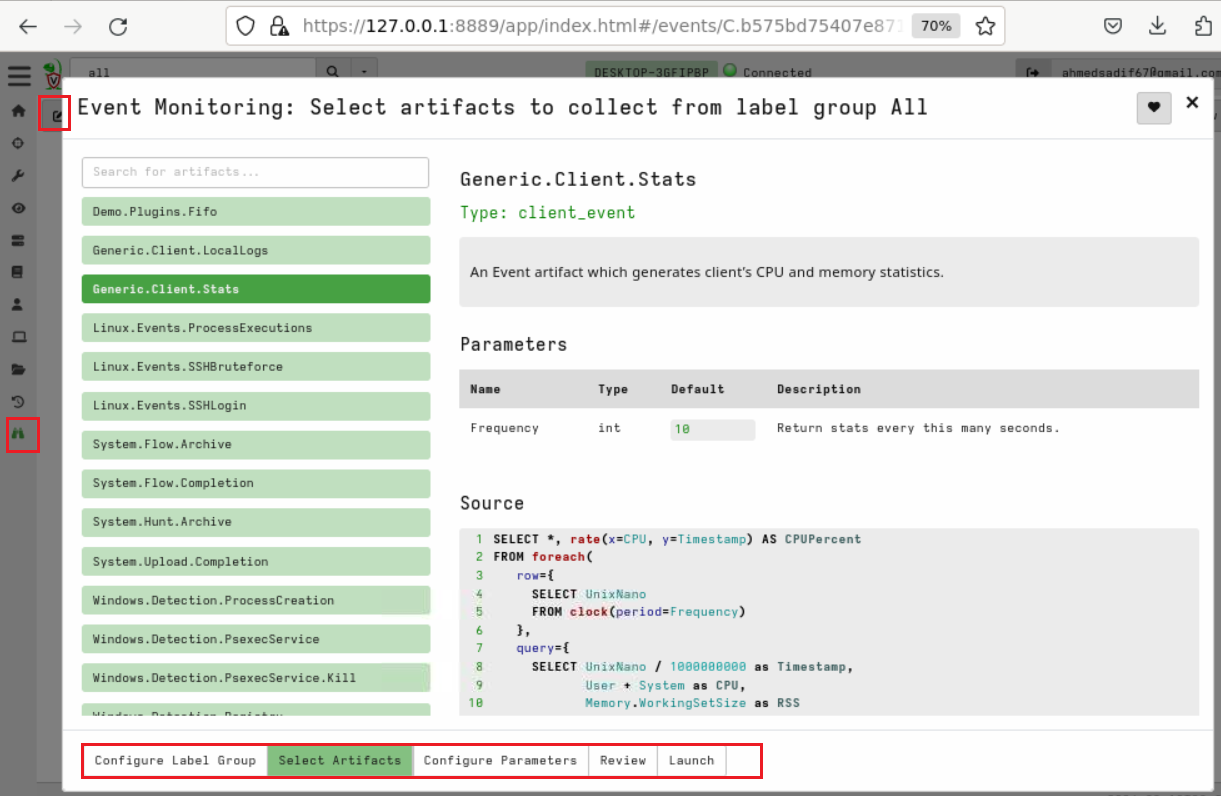
\includegraphics[width=\linewidth, center]{img/forensic/log1.png}
        \label{fig:log1}
    \end{subfigure}
    \begin{subfigure}{0.45\linewidth}
        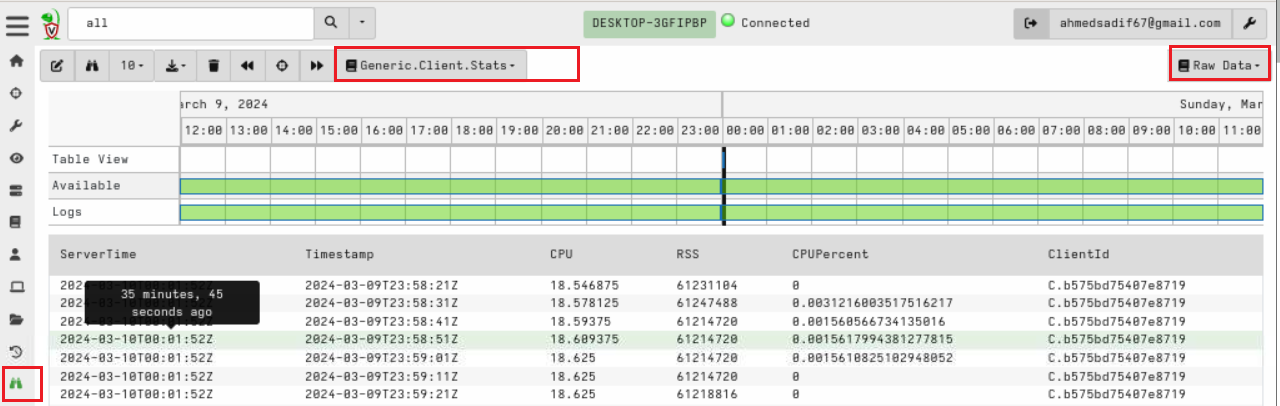
\includegraphics[width=\linewidth, center]{img/forensic/log2.png}
        \label{fig:log2}
    \end{subfigure}

    \caption{Client Side Event Queries}
    \label{fig:log}
\end{figure}
   
In the client, there can be many event watchers: queries that simply do not terminate. Besides \verb|watch_etw()|, there are \verb|watch_evtx()|, \verb|watch_usn()| etc. plugins to monitor changes in system. Collected events can be further processed in server side event queries.
\subsection{Incident Handling}
Often, investigators have to respond to incidents by first quickly determining relevant endpoints to an incident and then do a full collection from the selected endpoints, after isolating them. Velociraptor facilitates this through both the server client model and in non connected endpoints too. Following are some of the ways to handle incidents using Velociraptor.
\begin{figure}[ht]
    \centering
    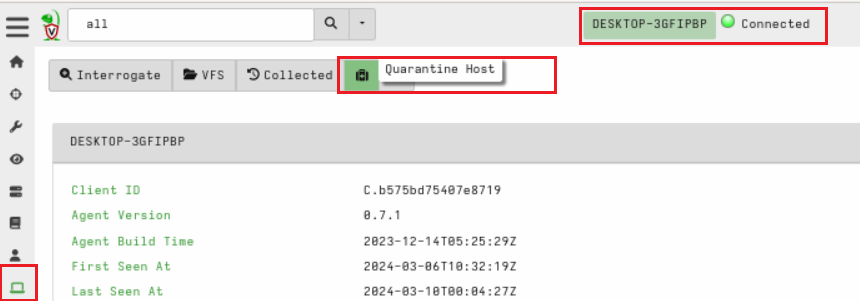
\includegraphics[width=\linewidth, center]{img/handling/quar1.png}
    \caption{Isolating A Single Endpoint}
    \label{fig:quar1}
\end{figure}

\subsubsection{Collection and Upload}
\verb|Windows.KapeFiles.Targets| is a very common collection artifact (\ref{artifacts}) for collecting various machine state data: registry, \verb|$MFT| table, process memories etc. User should monitor the collection resources while using this as collections usually exceed default resource values. The \verb|upload()| plugin(\ref{upload}) can be used to upload collections to server.

\subsubsection{Offline Collectors}
Often it may happen that a closed system needs investigation or the affected system is decided to be kept offline. Velociraptor can create offline collector executables that can be run simply to collect necessary files.
\begin{figure}[ht]
    \centering
    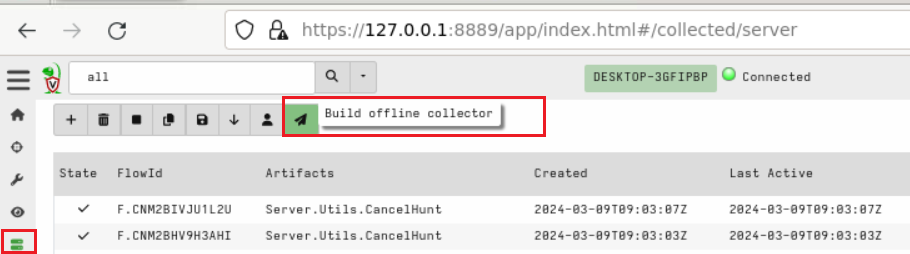
\includegraphics[width=\textwidth, center]{img/handling/coll1.png}
    \caption{Offline Collector Executable Creation}
    \label{fig:coll1}
\end{figure}

The collected zip file can be configured to be auto uploaded to a cloud storage such as AWS buckets. Or it could be imported as collection in the server using \verb|Server.Utils.ImportCollection| artifact. Like normal Velociraptor executables, this collector can also take command line arguments and even VQL queries(\ref{vql}) and execute them while collecting.

\section{Conclusion}
Velociraptor offers an unique solution to DFIR in a networked environment. However its core remains a simple, fast query engine. Thus by itself, a single instance can be an excellent collector and when deployed in network, Velociraptor is a fast, lightweight, versatile DFIR and monitoring tool. 
\section{References}
\begin{enumerate}
    \item \href{https://Github.com/Velocidex/velociraptor/}{Velociraptor Official Github Repository}
    \item \href{https://docs.velociraptor.app}{Velociraptor Official Documentation}
\end{enumerate}
\end{document}